%%%%%%%%%%%%%%%%%%%%%%%%%%%%%%%%%%%%%%%%%
% fphw Assignment
% LaTeX Template
% Version 1.0 (27/04/2019)
%
% This template originates from:
% https://www.LaTeXTemplates.com
%
% Authors:
% Class by Felipe Portales-Oliva (f.portales.oliva@gmail.com) with template 
% content and modifications by Vel (vel@LaTeXTemplates.com)
%
% Template (this file) License:
% CC BY-NC-SA 3.0 (http://creativecommons.org/licenses/by-nc-sa/3.0/)
%
%%%%%%%%%%%%%%%%%%%%%%%%%%%%%%%%%%%%%%%%%

%----------------------------------------------------------------------------------------
%	PACKAGES AND OTHER DOCUMENT CONFIGURATIONS
%----------------------------------------------------------------------------------------

\documentclass[
	12pt, % Default font size, values between 10pt-12pt are allowed
	%letterpaper, % Uncomment for US letter paper size
	%spanish, % Uncomment for Spanish
]{fphw}

% Template-specific packages
\usepackage[utf8]{inputenc} % Required for inputting international characters
\usepackage[T1]{fontenc} % Output font encoding for international characters
\usepackage{mathpazo} % Use the Palatino font
\usepackage[dvipsnames]{xcolor}
\usepackage{graphicx} % Required for including images
\usepackage{amsmath}
\usepackage{booktabs} % Required for better horizontal rules in tables
\usepackage{listings} % Required for insertion of code
\usepackage{enumerate} % To modify the enumerate environment
\usepackage{ragged2e}
\usepackage{cancel}
\usepackage{MnSymbol,bbding,pifont}
\usepackage{lscape}
\usepackage{array}
\usepackage{float,graphicx}
\newcolumntype{M}{>{$}c<{$}}
%----------------------------------------------------------------------------------------
%	ASSIGNMENT INFORMATION
%----------------------------------------------------------------------------------------

\title{Assignment \#2} % Assignment title

\author{Luis Alberto Ballado Aradias} % Student name

\date{\today} % Due date

\institute{Centro de Investigación y de Estudios Avanzados del IPN \\ Unidad Tamaulipas} % Institute or school name

\class{Tecnologías Computacionales (Sep - Dec 2022)} % Course or class name

\professor{Dr. Edwin Aldana Bobadilla} % Professor or teacher in charge of the assignment

%----------------------------------------------------------------------------------------

\begin{document}

\maketitle % Output the assignment title, created automatically using the information in the custom commands above

%----------------------------------------------------------------------------------------
%	ASSIGNMENT CONTENT
%----------------------------------------------------------------------------------------
{\color{teal}
\dotfill
BNF Notation
\dotfill}

BNF is a formal mathematical way of defining syntax unambiguosly.

It consists of:
\begin{itemize}
\item A set of terminal symbols
\item A set of non-terminal symbols
\item A set of production rules
\end{itemize}

LHS::= RHS ,LHS - LeftHandSide, ::= - is defined by, RHS - RightHandSide\\

Note: The LHS is always a non terminal symbol and The RHS is a sequence of symbols (terminals or non terminals)\\

for exmaple:
\[<DIGIT>::= 0|1|2|3|4|5|6|7|8|9\]

A letter can then be defined as:
\[<LETTER>::=A|B|C|D|E|......|Z\]
\[<WORD>::=<LETTER>|<LETTER><WORD>\]

So this now means a \textbf{word} is a single letter or a \textbf{letter} and a \textbf{word}\\

\begin{table}[ht]
\begin{tabular}{l l}
<> & Non terminal\\
::= & Produce\\
| & Alternative
\end{tabular}
\end{table}

Expressions\\
\begin{table}[ht]
\begin{tabular}{l l}
$\left[\right]$ & Optional\\
{} & Repetition\\
$A \dots \beta$ & rangos
\end{tabular}
\end{table}

\textbf{Why is Backus-Naur form needed?}\\

Can we create and apply BNF to describe the rules of a language?\\
\begin{itemize}
\item \textbf{Grammar:} Syntax and structure of a language.
\item \textbf{Natural Language:} a language that has developed naturally through use. (like Spanish, English .. etc).
\end{itemize}

BNF is a meta language - a language to describe another languages.\\
Need for Meta Languages:\\
\begin{itemize}
\item Determine whether a series of characters is valid
\item Generate well-formed statements
\item Break down a statement into constituent parts so it can be converted into machine code
\end{itemize}

BNF Deals with Terminals and Non-terminals
\begin{itemize}
\item Terminals: Symbols that can appear in the output of a language because of its rules, but cannot be changed by the rules themselves.
\item Non-terminals: Syntactic entities that define a part of the grammar (can be change by the rules).
\end{itemize}

\[<DIGIT>::= 0|1|2|3|4|5|6|7|8|9\]
In the previuos example Non-terminals is <DIGIT>, and the Terminals al the possible numbers a digit can be\\

We already know that \textbf{regular expressions} can be used to help us describe a simple language by specifying patterns of strings which match conditions.\\

Many aspects of languages can be defined using \textbf{regular expressions}, but it is both lengthy and time consuming.\\

Some aspects of languages such as the use of nested brackets cannot be difined using \textbf{regular expressions} at all, so we turn to meta-languages and Backus-Naur Form is an example of a meta language.


\section*{{\color{Apricot}BNF Notation in Python}}
%------------------------------------------------

\begin{verbatim}
ets may not.
star_targets:
    | star_target !','
    | star_target (',' star_target )* [',']
    star_targets_list_seq: ','.star_target+ [',']
    star_targets_tuple_seq:
    | star_target (',' star_target )+ [',']
    | star_target ','
    star_target:
    | '*' (!'*' star_target)
    | target_with_star_atom
    target_with_star_atom:
    | t_primary '.' NAME !t_lookahead
    | t_primary '[' slices ']' !t_lookahead
    | star_atom
    star_atom:
    | NAME
    | '(' target_with_star_atom ')'
    | '(' [star_targets_tuple_seq] ')'
    | '[' [star_targets_list_seq] ']'

    single_target:
    | single_subscript_attribute_target
    | NAME
    | '(' single_target ')'
    single_subscript_attribute_target:
    | t_primary '.' NAME !t_lookahead
    | t_primary '[' slices ']' !t_lookahead

    del_targets: ','.del_target+ [',']
    del_target:
    | t_primary '.' NAME !t_lookahead
    | t_primary '[' slices ']' !t_lookahead
    | del_t_atom
    del_t_atom:
    | NAME
    | '(' del_target ')'
    | '(' [del_targets] ')'
    | '[' [del_targets] ']'

    t_primary:
    | t_primary '.' NAME &t_lookahead
    | t_primary '[' slices ']' &t_lookahead
    | t_primary genexp &t_lookahead
    | t_primary '(' [arguments] ')' &t_lookahead
    | atom &t_lookahead
    t_lookahead: '(' | '[' | '.'
  
\end{verbatim}
%----------------------------------------------------------------------------------------

\section*{{\color{ForestGreen}BNF Notation in C}}
%------------------------------------------------
\begin{verbatim}
<translation-unit> ::= {<external-declaration>}*

<external-declaration> ::= <function-definition>
                         | <declaration>

<function-definition> ::= {<declaration-specifier>}* <declarator> {<declaration>}* <compound-statement>

<declaration-specifier> ::= <storage-class-specifier>
                          | <type-specifier>
                          | <type-qualifier>

<storage-class-specifier> ::= auto
                            | register
                            | static
                            | extern
                            | typedef

<type-specifier> ::= void
                   | char
                   | short
                   | int
                   | long
                   | float
                   | double
                   | signed
                   | unsigned
                   | <struct-or-union-specifier>
                   | <enum-specifier>
                   | <typedef-name>

<struct-or-union-specifier> ::= <struct-or-union> <identifier> { {<struct-declaration>}+ }
                              | <struct-or-union> { {<struct-declaration>}+ }
                              | <struct-or-union> <identifier>

<struct-or-union> ::= struct
                    | union

<struct-declaration> ::= {<specifier-qualifier>}* <struct-declarator-list>

<specifier-qualifier> ::= <type-specifier>
                        | <type-qualifier>

<struct-declarator-list> ::= <struct-declarator>
                           | <struct-declarator-list> , <struct-declarator>

<struct-declarator> ::= <declarator>
                      | <declarator> : <constant-expression>
                      | : <constant-expression>

<declarator> ::= {<pointer>}? <direct-declarator>

<pointer> ::= * {<type-qualifier>}* {<pointer>}?

<type-qualifier> ::= const
                   | volatile

<direct-declarator> ::= <identifier>
                      | ( <declarator> )
                      | <direct-declarator> [ {<constant-expression>}? ]
                      | <direct-declarator> ( <parameter-type-list> )
                      | <direct-declarator> ( {<identifier>}* )

<constant-expression> ::= <conditional-expression>

<conditional-expression> ::= <logical-or-expression>
                           | <logical-or-expression> ? <expression> : <conditional-expression>

<logical-or-expression> ::= <logical-and-expression>
                          | <logical-or-expression> || <logical-and-expression>

<logical-and-expression> ::= <inclusive-or-expression>
                           | <logical-and-expression> && <inclusive-or-expression>

<inclusive-or-expression> ::= <exclusive-or-expression>
                            | <inclusive-or-expression> | <exclusive-or-expression>

<exclusive-or-expression> ::= <and-expression>
                            | <exclusive-or-expression> ^ <and-expression>

<and-expression> ::= <equality-expression>
                   | <and-expression> & <equality-expression>

<equality-expression> ::= <relational-expression>
                        | <equality-expression> == <relational-expression>
                        | <equality-expression> != <relational-expression>

<relational-expression> ::= <shift-expression>
                          | <relational-expression> < <shift-expression>
                          | <relational-expression> > <shift-expression>
                          | <relational-expression> <= <shift-expression>
                          | <relational-expression> >= <shift-expression>

<shift-expression> ::= <additive-expression>
                     | <shift-expression> << <additive-expression>
                     | <shift-expression> >> <additive-expression>

<additive-expression> ::= <multiplicative-expression>
                        | <additive-expression> + <multiplicative-expression>
                        | <additive-expression> - <multiplicative-expression>

<multiplicative-expression> ::= <cast-expression>
                              | <multiplicative-expression> * <cast-expression>
                              | <multiplicative-expression> / <cast-expression>
                              | <multiplicative-expression> % <cast-expression>

<cast-expression> ::= <unary-expression>
                    | ( <type-name> ) <cast-expression>

<unary-expression> ::= <postfix-expression>
                     | ++ <unary-expression>
                     | -- <unary-expression>
                     | <unary-operator> <cast-expression>
                     | sizeof <unary-expression>
                     | sizeof <type-name>

<postfix-expression> ::= <primary-expression>
                       | <postfix-expression> [ <expression> ]
                       | <postfix-expression> ( {<assignment-expression>}* )
                       | <postfix-expression> . <identifier>
                       | <postfix-expression> -> <identifier>
                       | <postfix-expression> ++
                       | <postfix-expression> --

<primary-expression> ::= <identifier>
                       | <constant>
                       | <string>
                       | ( <expression> )

<constant> ::= <integer-constant>
             | <character-constant>
             | <floating-constant>
             | <enumeration-constant>

<expression> ::= <assignment-expression>
               | <expression> , <assignment-expression>

<assignment-expression> ::= <conditional-expression>
                          | <unary-expression> <assignment-operator> <assignment-expression>

<assignment-operator> ::= =
                        | *=
                        | /=
                        | %=
                        | +=
                        | -=
                        | <<=
                        | >>=
                        | &=
                        | ^=
                        | |=

<unary-operator> ::= &
                   | *
                   | +
                   | -
                   | ~
                   | !

<type-name> ::= {<specifier-qualifier>}+ {<abstract-declarator>}?

<parameter-type-list> ::= <parameter-list>
                        | <parameter-list> , ...

<parameter-list> ::= <parameter-declaration>
                   | <parameter-list> , <parameter-declaration>

<parameter-declaration> ::= {<declaration-specifier>}+ <declarator>
                          | {<declaration-specifier>}+ <abstract-declarator>
                          | {<declaration-specifier>}+

<abstract-declarator> ::= <pointer>
                        | <pointer> <direct-abstract-declarator>
                        | <direct-abstract-declarator>

<direct-abstract-declarator> ::=  ( <abstract-declarator> )
                               | {<direct-abstract-declarator>}? [ {<constant-expression>}? ]
                               | {<direct-abstract-declarator>}? ( {<parameter-type-list>}? )

<enum-specifier> ::= enum <identifier> { <enumerator-list> }
                   | enum { <enumerator-list> }
                   | enum <identifier>

<enumerator-list> ::= <enumerator>
                    | <enumerator-list> , <enumerator>

<enumerator> ::= <identifier>
               | <identifier> = <constant-expression>

<typedef-name> ::= <identifier>

<declaration> ::=  {<declaration-specifier>}+ {<init-declarator>}* ;

<init-declarator> ::= <declarator>
                    | <declarator> = <initializer>

<initializer> ::= <assignment-expression>
                | { <initializer-list> }
                | { <initializer-list> , }

<initializer-list> ::= <initializer>
                     | <initializer-list> , <initializer>

<compound-statement> ::= { {<declaration>}* {<statement>}* }

<statement> ::= <labeled-statement>
              | <expression-statement>
              | <compound-statement>
              | <selection-statement>
              | <iteration-statement>
              | <jump-statement>

<labeled-statement> ::= <identifier> : <statement>
                      | case <constant-expression> : <statement>
                      | default : <statement>

<expression-statement> ::= {<expression>}? ;

<selection-statement> ::= if ( <expression> ) <statement>
                        | if ( <expression> ) <statement> else <statement>
                        | switch ( <expression> ) <statement>

<iteration-statement> ::= while ( <expression> ) <statement>
                        | do <statement> while ( <expression> ) ;
                        | for ( {<expression>}? ; {<expression>}? ; {<expression>}? ) <statement>

<jump-statement> ::= goto <identifier> ;
                   | continue ;
                   | break ;
                   | return {<expression>}? ;
\end{verbatim}
%----------------------------------------------------------------------------------------

\section*{{\color{Cerulean}BNF Notation in Java}}
%------------------------------------------------
\begin{verbatim}
compilation_unit  = 
 [ package_statement ] 
 < import_statement > 
 < type_declaration >  . 

package_statement  = 
 "package" package_name  ";"  . 

import_statement  = 
 "import"  (  ( package_name  "."  "*"  ";"  ) 
 /  ( class_name  / interface_name )  )  ";"  . 

type_declaration  = 
 [ doc_comment ]  ( class_declaration  / interface_declaration )  ";"  . 

doc_comment  =  "/**"  "... text ..."  "*/"  . 

class_declaration  = 
 < modifier >  "class" identifier 
 [  "extends" class_name ] 
 [  "implements" interface_name  <  "," interface_name >  ] 
 "{"  < field_declaration >  "}"  . 

interface_declaration  = 
 < modifier >  "interface" identifier 
 [  "extends" interface_name  <  "," interface_name >  ] 
 "{"  < field_declaration >  "}"  . 

field_declaration  = 
 (  [ doc_comment ]  ( method_declaration 
 / constructor_declaration 
 / variable_declaration )  ) 
 / static_initializer 
 /  ";"  . 

method_declaration  = 
 < modifier > type identifier 
 "("  [ parameter_list ]  ")"  <  "["  "]"  > 
 ( statement_block  /  ";"  )  . 

constructor_declaration  = 
 < modifier > identifier  "("  [ parameter_list ]  ")" 
statement_block  . 

statement_block  =  "{"  < statement >  "}"  . 

variable_declaration  = 
 < modifier > type variable_declarator 
 <  "," variable_declarator  >  ";"  . 

variable_declarator  = 
 identifier  <  "["  "]"  >  [  "=" variable_initializer ]  . 

variable_initializer  = 
expression 
 /  (  "{"  [ variable_initializer 
 <  "," variable_initializer  >  [  ","  ]  ]  "}"  )  . 

static_initializer  = 
 "static" statement_block  . 

parameter_list  = 
parameter  <  "," parameter >  . 

parameter  = 
type identifier  <  "["  "]"  >  . 

statement  = 
variable_declaration 
 /  ( expression  ";"  ) 
 /  ( statement_block ) 
 /  ( if_statement ) 
 /  ( do_statement ) 
 /  ( while_statement ) 
 /  ( for_statement ) 
 /  ( try_statement ) 
 /  ( switch_statement ) 
 /  (  "synchronized"  "(" expression  ")" statement  ) 
 /  (  "return"  [ expression ]  ";"  ) 
 /  (  "throw" expression ";"  ) 
 /  ( identifier  ":" statement ) 
 /  (  "break"  [ identifier ]  ";"  ) 
 /  (  "continue"  [ identifier ]  ";"  ) 
 /  (  ";"  )  . 

if_statement = 
 "if"  "(" expression  ")" statement 
 [  "else" statement ]  . 

do_statement = 
 "do" statement  "while"  "(" expression  ")"  ";"  . 

while_statement = 
 "while"  "(" expression  ")" statement  . 

for_statement = 
 "for"  "("  ( variable_declaration  /  ( expression  ";"  )  /  ";"  ) 
 [ expression ]  ";" 
 [ expression ]  ";" 
 ")" statement  . 

try_statement = 
 "try" statement 
 <  "catch"  "(" parameter  ")" statement > 
 [  "finally" statement ]  . 

switch_statement = 
 "switch"  "(" expression  ")"  "{" 
 <  (  "case" expression  ":"  ) 
 /  (  "default"  ":"  ) 
 / statement > 
 "}"  . 

expression  = 
numeric_expression 
 / testing_expression 
 / logical_expression 
 / string_expression 
 / bit_expression 
 / casting_expression 
 / creating_expression 
 / literal_expression 
 /  "null" 
 /  "super" 
 /  "this" 
 / identifier 
 /  (  "(" expression  ")"  ) 
 /  ( expression 
 (  (  "("  [ arglist ]  ")"  ) 
 /  (  "[" expression  "]"  ) 
 /  (  "." expression  ) 
 /  (  "," expression  ) 
 /  (  "instanceof"  ( class_name / interface_name )  ) 
 )  )  . 

numeric_expression  = 
 (  (  "-" 
 /  "++" 
 /  "--"  ) 
expression ) 
 /  ( expression 
 (  "++" 
 /  "--"  )  ) 
 /  ( expression 
 (  "+" 
 /  "+=" 
 /  "-" 
 /  "-=" 
 /  "*" 
 /  "*=" 
 /  "/" 
 /  "/=" 
 /  "%" 
 /  "%="  ) 
expression  )  . 

testing_expression  = 
 ( expression 
 (  ">" 
 /  "<" 
 /  ">=" 
 /  "<=" 
 /  "==" 
 /  "!="  ) 
expression  )  . 

logical_expression  = 
 (  "!" expression ) 
 /  ( expression 
 (  "ampersand" 
 /  "ampersand=" 
 /  "|" 
 /  "|=" 
 /  "^" 
 /  "^=" 
 /  (  "ampersand"  "ampersand"  ) 
 /  "||=" 
 /  "%" 
 /  "%="  ) 
expression  ) 
 /  ( expression  "?" expression  ":" expression ) 
 /  "true" 
 /  "false"  . 

string_expression  =  ( expression 
 (  "+" 
 /  "+="  ) 
expression  )  . 

bit_expression  = 
 (  "~" expression ) 
 /  ( expression 
 (  ">>=" 
 /  "<<" 
 /  ">>" 
 /  ">>>"  ) 
expression  )  . 

casting_expression  = 
 "(" type  ")" expression  . 

creating_expression  = 
 "new"  (  ( classe_name  "("  [ arglist ]  ")"  ) 
 /  ( type_specifier  [  "[" expression  "]"  ]  <  "["  "]"  >  ) 
 /  (  "(" expression  ")"  )  )  . 

literal_expression  = 
integer_literal 
 / float_literal 
 / string 
 / character  . 

arglist  = 
expression  <  "," expression  >  . 

type  = 
type_specifier  <  "["  "]"  >  . 

type_specifier = 
 "boolean" 
 /  "byte" 
 /  "char" 
 /  "short" 
 /  "int" 
 /  "float" 
 /  "long" 
 /  "double" 
 / class_name 
 / interface_name  . 

modifier = 
 "public" 
 /  "private" 
 /  "protected" 
 /  "static" 
 /  "final" 
 /  "native" 
 /  "synchronized" 
 /  "abstract" 
 /  "threadsafe" 
 /  "transient"  . 

package_name = 
identifier 
 /  ( package_name  "." identifier )  . 

class_name  = 
identifier 
 /  ( package_name  "." identifier )  . 

interface_name = 
identifier 
 /  ( package_name  "." identifier )  . 

integer_literal = 
 (  (  "1..9"  <  "0..9"  >  ) 
 /  <  "0..7"  > 
 /  (  "0"  "x"  "0..9a..f"  <  "0..9a..f"  >  )  ) 
 [  "l"  ]  . 

float_literal  = 
 ( decimal_digits  "."  [ decimal_digits ]  [ exponent_part ]  [ float_type_suffix ]  ) 
 /  (  "." decimal_digits  [ exponent_part ]  [ float_type_suffix ]  ) 
 /  ( decimal_digits  [ exponent_part ]  [ float_type_suffix ]  )  . 

decimal_digits  = 
 "0..9"  <  "0..9"  >  . 

exponent_part  = 
 "e"  [  "+"  /  "-"  ] decimal_digits  . 

float_type_suffix  = 
 "f"  /  "d"  . 

character  =
  "based on the unicode character set"  . 

string  =  
 "''"  < character  >  "''"  . 

identifier  =
  "a..z,$,_"  <  "a..z,$,_,0..9,unicode character over 00C0"  >  . 

\end{verbatim}

%----------------------------------------------------------------------------------------

\section*{{\color{RoyalPurple}BNF Notation inSQL}}
%------------------------------------------------

\begin{figure}[H]
  \centering
  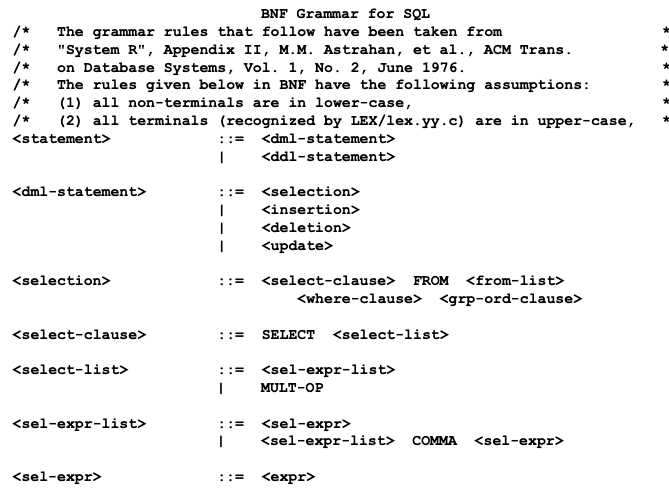
\includegraphics[scale=0.7]{images/bnf1.png}
\end{figure}
\begin{figure}[H]
  \centering
  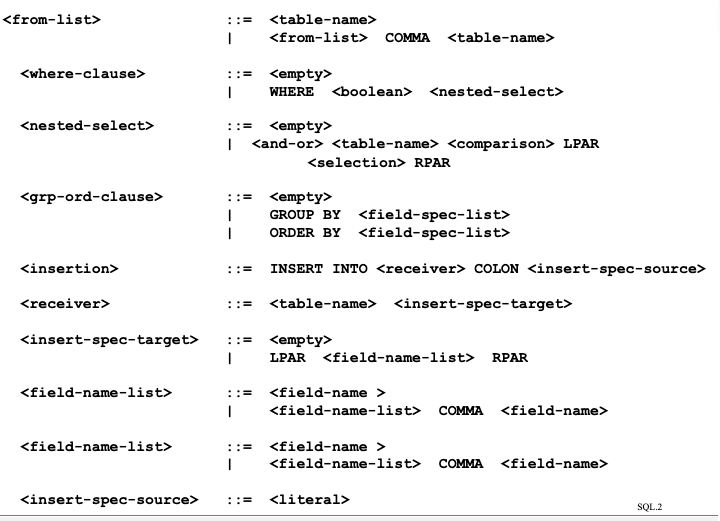
\includegraphics[scale=0.7]{images/bnf2.png}
\end{figure}
\begin{figure}[H]
  \centering
  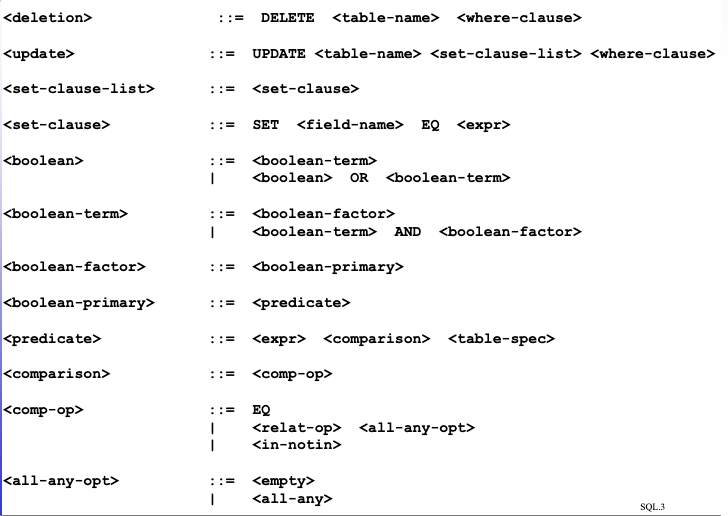
\includegraphics[scale=0.7]{images/bnf3.png}
\end{figure}
\begin{figure}[H]
  \centering
  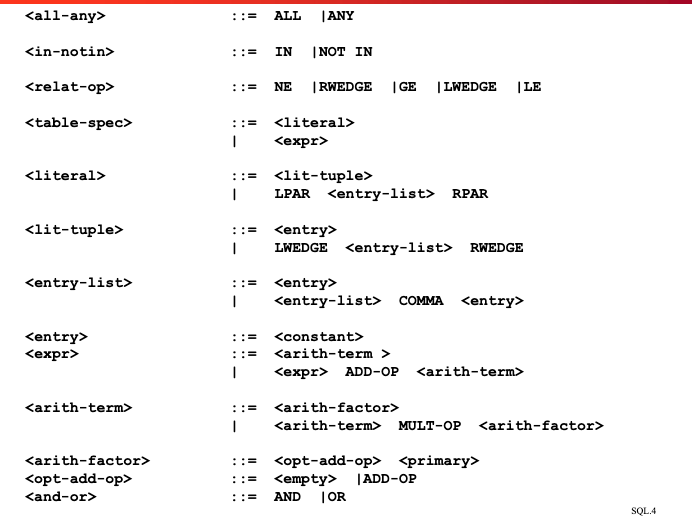
\includegraphics[scale=0.7]{images/bnf4.png}
\end{figure}
\begin{figure}[H]
  \centering
  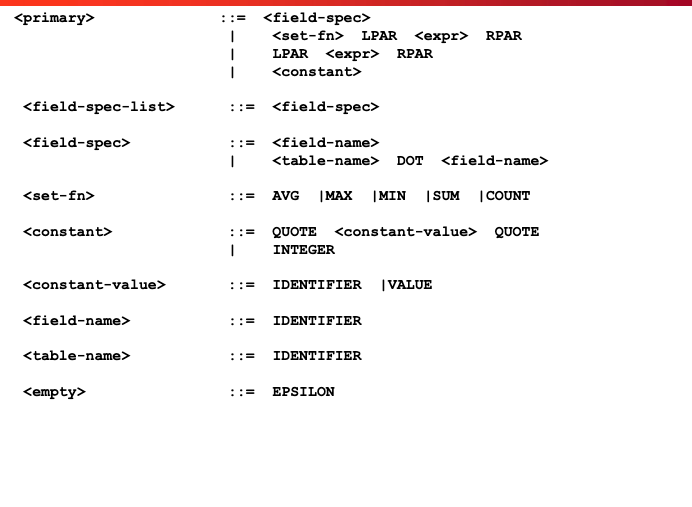
\includegraphics[scale=0.7]{images/bnf5.png}
\end{figure}
\begin{figure}[H]
  \centering
  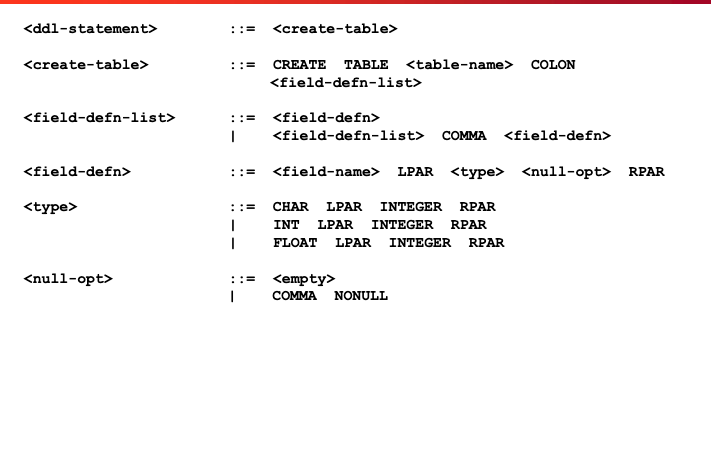
\includegraphics[scale=0.7]{images/bnf6.png}
\end{figure}

%----------------------------------------------------------------------------------------

\end{document}
